% !TEX root = slides.tex

\begin{frame}[t]
\label{bayespc_m}
\frametitle{In a different language....}
\small
\vspace*{-3mm}

\bri

\item $N$ training data points $(\vxi_i,Z_i)$ and $K+1$ basis terms $\Psi_k(\cdot)$
\item `Measurement' matrix $\vP^{N\times (K+1)}$ with $\vP_{ik}=\Psi_k(\vxi_i)$
\item Find regression weights $\vc=(c_0,\dots,c_{K})$ so that
\eri
\begin{center}


\begin{tikzpicture} \node [rounded corners,fill=blue!10] {
$\vZ\approx \vP \vc $
};
\end{tikzpicture}
$\qquad\qquad$ \textrm{   or   } $\qquad\qquad$
 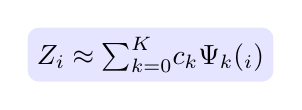
\begin{tikzpicture} \node [rounded corners,fill=blue!10] {
$ Z_i \approx{\sum_{k=0}^K} c_k \Psi_k(\vxi_i)$
};
\end{tikzpicture}
\end{center}
\vspace*{-0.3cm}
\bri
\item The number of polynomial basis terms grows fast; a $p$-th order, $d$-dimensional basis has a total of $K+1=(p+d)!/(p!d!)$ terms.
\item For limited data and large basis set ($N\le K$) this is a sparse
  signal recovery problem $\Rightarrow$ need some regularization/constraints.
\eri

\bbi
\item Least-squares $\qquad\qquad\argmin_{\vc} \left\{||\vZ-\vP\vc||^2_2\right\}$
\vspace*{0.3cm}
\item The `sparsest'       $\qquad\qquad\argmin_{\vc} \left\{||\vZ-\vP\vc||^2_2+\alpha||\vc||_0\right\}$
\vspace*{0.3cm}
\item Compressive sensing  $\qquad\qquad\argmin_{\vc} \left\{||\vZ-\vP\vc||^2_2+\alpha||\vc||_1\right\}$
% \only<2>{
% \begin{blue}\footnotesize{\hspace*{1cm} Bayesian \hspace*{3.8cm} Likelihood \hspace*{0.5cm} Prior}\end{blue}
% }
\ebi

%\only<2->{
%\bbi
%\item Tikhonov regularization $\qquad\qquad\textit{argmin}_{\vc} \left\{||\vy-\vP\vc||_2+\alpha||\vc||_2\right\}$
%\vspace*{0.3cm}
%\item Lasso regression        $\qquad\qquad\textit{argmin}_{\vc} \left\{||\vy-\vP\vc||_2\right\}$ subject to $||\vc||_1\le \alpha$
%\vspace*{0.3cm}
%\item Compressive sensing  $\qquad\qquad\textit{argmin}_{\vc} \left\{||\vy-\vP\vc||_2+\alpha||\vc||_1\right\}$
%\only<3>{
%\begin{blue}\footnotesize{\hspace*{1cm} Bayesian \hspace*{3.8cm} Likelihood \hspace*{0.5cm} Prior}\end{blue}
%}
%\ebi
%}




\end{frame}


